%=================================================================
\documentclass[entropy,article,submit,pdftex,oneauthor]{Definitions/mdpi}
%=================================================================

%=================================================================
% MDPI internal commands - do not modify
\firstpage{1}
\makeatletter
\setcounter{page}{\@firstpage}
\makeatother
\pubvolume{1}
\issuenum{1}
\articlenumber{0}
\pubyear{2025}
\copyrightyear{2025}
%\externaleditor{Firstname Lastname}
\datereceived{ }
\daterevised{ } % Comment out if no revised date
\dateaccepted{ }
\datepublished{ }
\hreflink{https://doi.org/10.5281/zenodo.16616699}
%\doinum{}
%\pdfoutput=1
%\CorrStatement{yes}
%\longauthorlist{yes}

%=================================================================
% Packages (kept minimal; class already loads many)
\usepackage{amsmath, amssymb}
\usepackage{tcolorbox}
\usepackage{physics}
\usepackage{bm}
\usetikzlibrary{knots,intersections,decorations.pathreplacing,3d,calc,arrows.meta,positioning,decorations.pathmorphing}
\usepackage{pgfmath}
\usepackage{pgfplots}
\pgfplotsset{compat=1.18}
\usepackage{lmodern}
\usepackage{mathtools}
\usepackage[normalem]{ulem}

%=================================================================
%====================  Rosetta v0.6 / Canon macro layer (aliases)  ====================
% Safe fallbacks (no-ops if already defined)
\providecommand{\rhoF}{\rho_{\!f}}
\providecommand{\rhoE}{\rho_{\!E}}
\providecommand{\rhoM}{\rho_{\!m}}
\providecommand{\rhoC}{\rho_{\text{core}}}
\providecommand{\rc}{r_c}
\providecommand{\vswirl}{\mathbf{v}_{\!\boldsymbol{\circlearrowleft}}}
\providecommand{\vnorm}{\lVert\vswirl\rVert}
\providecommand{\vomega}{\boldsymbol{\omega}}
\providecommand{\Rloc}{R}

%---- Time hierarchy (canonical symbols) ----
\providecommand{\Nabs}{\mathcal{N}}          % absolute foliation time
\providecommand{\nuZero}{\nu_{0}}            % baseline phase / reference rate
\providecommand{\ptau}{\tau}                 % proper time
\providecommand{\Sswirl}{S^{\circlearrowleft}_{\!(t)}} % internal swirl clock
\providecommand{\Tv}{T_{v}}                  % observed time layer
\providecommand{\Ktop}{\mathbb{K}}           % topological time

% Readable aliases (use anywhere in prose or math)
\providecommand{\AbsTime}{\Nabs}
\providecommand{\ProperTime}{\ptau}
\providecommand{\SwirlClock}{\Sswirl}
\providecommand{\ObservedTime}{\Tv}
\providecommand{\TopoTime}{\Ktop}

%---- Swirl clock factor and related helpers ----
% S_t symbol and a typed version that expands the analytic form
\providecommand{\St}{S_{t}}
\providecommand{\StOf}[1]{\sqrt{\,1-\dfrac{#1^{\,2}}{c^{2}}\,}} % #1 := tangential speed

% Tangential swirl speed choices (pick one in text)
%   \vt := |v_swirl| ; or \vtAng := |\omega| R
\providecommand{\vt}{\vnorm}
\providecommand{\vtAng}{\lvert\vomega\rvert\,\Rloc}

%---- Canonical numerical constants (typeset convenience only)
\providecommand{\VswirlConst}{1.09384563\times 10^{6}\,\mathrm{m\,s^{-1}}}
\providecommand{\rcConst}{1.40897017\times 10^{-15}\,\mathrm{m}}
\providecommand{\rhoCoreConst}{3.8934358266918687\times 10^{18}\,\mathrm{kg\,m^{-3}}}
\providecommand{\rhoFConst}{7.0\times 10^{-7}\,\mathrm{kg\,m^{-3}}}
\providecommand{\FswirlMax}{29.053507\,\mathrm{N}}
\providecommand{\FgravMax}{3.02563\times 10^{43}\,\mathrm{N}}

%---- Legacy text shields (optional): map leftover tokens to neutral phrasing
% Uncomment only if you still have macros for legacy terms.
% \providecommand{\Aether}{\text{structured space}}
% \providecommand{\Ether}{\text{structured space}}
% \providecommand{\Vortex}{\text{swirl}}
%======================================================================================


%=================================================================
% Title (Rosetta mainstream wording; no “\AE ther” or “Vortex”)
\Title{Revisiting Structured Space: From Einstein to a Swirl–String Framework}
\TitleCitation{Revisiting Structured Space}
\newcommand{\orcidauthorA}{0009-0006-1686-3961}
\Author{Omar Iskandarani $^{1}$\orcidA{}}
\AuthorNames{Omar Iskandarani}
\AuthorCitation{Iskandarani, O.}

% MDPI metadata block
\address{$^{1}$ \\ Independent Researcher, Groningen, The Netherlands;  info@omariskandarani.com}
\corres{Correspondence: info@omariskandarani.com}

%=================================================================
% Abstract — rewritten in Rosetta v0.6 mainstream language
\abstract{This paper revisits Einstein’s later remarks on a structured space and proposes a modern realization in a swirl–string framework with preferred foliation. The medium is modeled as an incompressible, inviscid condensate supporting quantized circulation along closed filaments (swirl strings). Gravitational and inertial phenomena arise from swirl-induced pressure gradients and coherent circulation, with local time scaling governed by the tangential swirl speed. Mass corresponds to localized topological tension, and attraction emerges from Bernoulli-like pressure deficits sustained by circulation invariants. The framework yields testable predictions for clock behavior, frame-dragging analogues, and vorticity-coupled fields, with analog implementations in superfluids and optical platforms. We argue that “structured space” is neither obsolete nor purely geometric: it is a dynamic, quantized substrate amenable to precise modeling and experiment.}

% Keywords — neutralized (no “\AE ther”, no “Vortex”)
\keyword{emergent gravity; topological fluid dynamics; analogue gravity; swirl strings; preferred foliation; time dilation; structured vacuum}

%%%%%%%%%%%%%%%%%%%%%%%%%%%%%%%%%%%%%%%%%%
\begin{document}
%%%%%%%%%%%%%%%%%%%%%%%%%%%%%%%%%%%%%%%%%%

%-----------------------------
    \section{Introduction}\label{sec:introduction}
        It is often claimed that Einstein “abolished the ether” in his theory of relativity. While this has become a popular shorthand in educational and philosophical discussions, it oversimplifies Einstein’s position~\cite{einstein1920aether}. In 1905, he dispensed with a mechanical carrier for electromagnetic waves; in later writings—most notably the 1920 Leiden address—he argued for a non-mechanical, structured space endowed with metric properties. For historical quotations and their mappings to dynamics in the present framework, see Appendix~\ref{appendix:einstein}.

        This paper revisits Einstein’s evolving perspective on structured space and evaluates its compatibility with a swirl–string framework grounded in a preferred foliation, as developed in the SST Canon and companion derivations~\cite{SST-Canon-0.5.10,SST-Canonical-Fluid}.

        In this framework, the underlying medium is modeled as incompressible and inviscid, with quantized circulation supported along closed filaments (“swirl strings”). Coherent circulation generates pressure gradients and inertial response; local time scaling follows the tangential swirl speed via the swirl clock factor. Mass corresponds to localized topological tension, and long-range attraction emerges from Bernoulli-type pressure deficits sustained by circulation invariants~\cite{SST-Canon-0.5.10,SST-Canonical-Fluid}.

        \textit{This formalism has been applied to the photon sector as an R-phase torsional excitation in a structured medium, providing a concrete model for electromagnetic propagation and quantized energy flow~\cite{SST-Canon-0.5.10,SST-Canonical-Fluid}.}

        We extend this ontology to spacetime kinematics and temporal structure, positioning the swirl–string program as a coherent alternative to purely geometric field-theoretic approaches~\cite{SST-Canonical-Fluid}.

        Through a topological–dynamical synthesis, the framework offers explicit, testable predictions that connect historical field theory to contemporary advances~\cite{SST-Canonical-Fluid,SST-Heat-Transport,SST-Hydrogen-Gravity}, and aligns with analogue-gravity programs where fluid systems mimic effective relativistic metrics~\cite{barcelo2005}. This trajectory is summarized in Figure~\ref{fig:history-temporal-ontology}, which maps milestones in the conceptualization of time—from classical notions and introspective accounts to relativized geometry and a layered temporality in filamentary circulation.

        \begin{figure}[htbp]
      \centering
    \scriptsize
    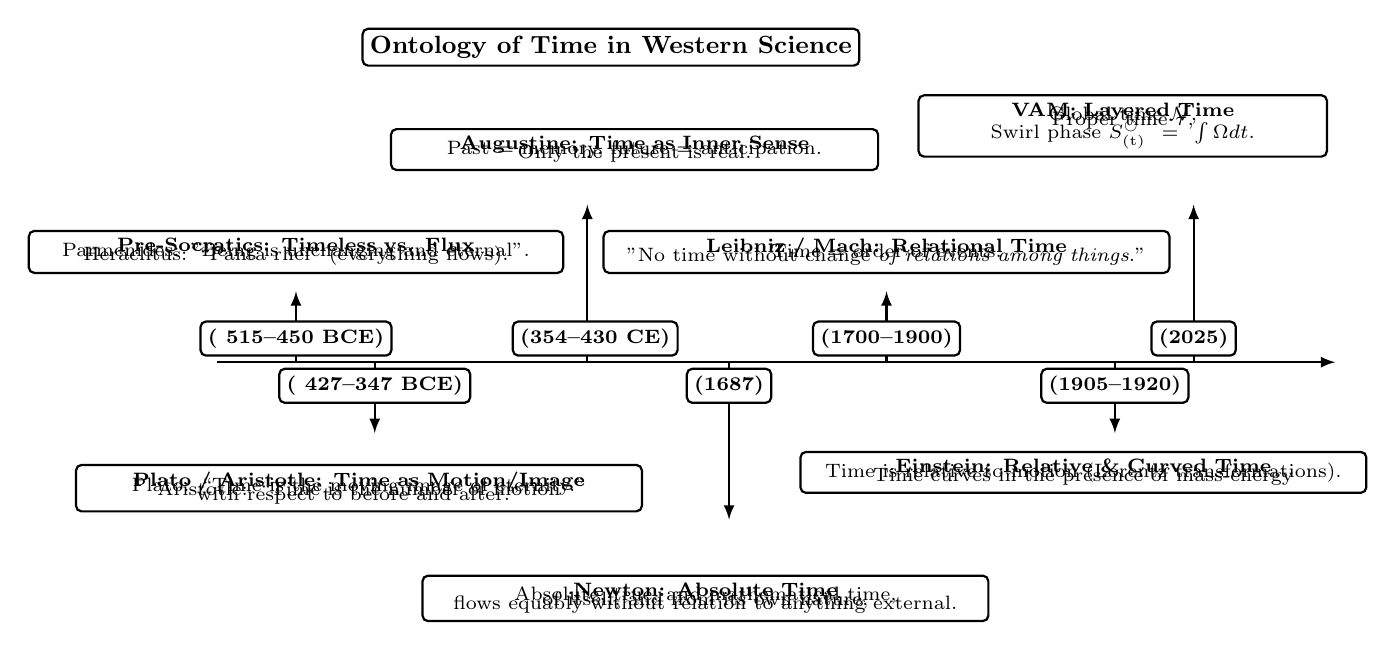
\begin{tikzpicture}[node distance=3.5cm, every node/.style={font=\scriptsize}, >=latex]
    \scriptsize

    % Timeline base
    \draw[->, thick] (-1,0) -- (13.2,0);

    % Arrows above timeline (short, as requested)
    \draw[->, thick] (0,0) -- (0,0.9);       % Pre-Socratics
    \draw[->, thick] (3.7,0) -- (3.7,2.0);   % Augustine
    \draw[->, thick] (7.5,0) -- (7.5,0.9);   % Einstein
    \draw[->, thick] (11.4,0) -- (11.4,2.0); % VAM

    % Arrows below timeline (short, as requested)
    \draw[->, thick] (1.0,0) -- (1.0,-0.9);     % Plato/Aristotle
    \draw[->, thick] (5.5,0) -- (5.5,-2.0);     % Newton
    \draw[->, thick] (10.4,0) -- (10.4,-0.9);     % Leibniz/Mach

        %--- Root title cards (above timeline) ---
    \node[draw, thick, rounded corners=2pt, fill=white, align=center, font=\bfseries ] at (0, .3)   {(~515–450 BCE)};
    \node[draw, thick, rounded corners=2pt, fill=white, align=center, font=\bfseries ] at (3.8, .3) {(354–430 CE)};
    \node[draw, thick, rounded corners=2pt, fill=white, align=center, font=\bfseries ] at (7.5, .3) {(1700--1900)};
    \node[draw, thick, rounded corners=2pt, fill=white, align=center, font=\bfseries ] at (11.4, .3){(2025)};

    %--- Root title cards (below timeline) ---
    \node[draw, thick, rounded corners=2pt, fill=white, align=center, font=\bfseries ] at (1.0,- .3) {(~427–347 BCE)};
    \node[draw, thick, rounded corners=2pt, fill=white, align=center, font=\bfseries ] at (5.5,- .3) {(1687)};
    \node[draw, thick, rounded corners=2pt, fill=white, align=center, font=\bfseries ] at (10.4,- .3) {(1905--1920)};

    % Label
    \node[draw, thick, fill=white, rounded corners=2pt, font=\small] at (4,4.0) {\textbf{Ontology of Time in Western Science}};

    % Ancient Greek: Parmenides / Heraclitus
    \node[draw, rounded corners=2pt, thick, align=center, fill=white, text width=6.6cm] at (0,1.4) {
    \textbf{Pre-Socratics: Timeless vs. Flux}  \\[-0.8em]
    Parmenides: "Being is unchanging and eternal".  \\[-0.8em]
    Heraclitus: “Panta rhei” (everything flows).
    };

    % Plato / Aristotle
    \node[draw, rounded corners=2pt, thick, align=center, fill=white, text width=7cm] at (0.8,-1.6) {
    \textbf{Plato / Aristotle: Time as Motion/Image}  \\[-0.8em]
    Plato: “Time is the moving image of eternity.” \\[-0.8em]
    Aristotle: “Time is the number of motion \\[-0.8em]
    with respect to before and after.”
    };

    % Augustine
    \node[draw, rounded corners=2pt, thick, align=center, fill=white, text width=6cm] at (4.3,2.7) {
    \textbf{Augustine: Time as Inner Sense}  \\[-0.8em]
    Past = memory, future = anticipation. \\[-0.8em]
    Only the present is real.
    };

    % Newton
    \node[draw, rounded corners=2pt, thick, align=center, fill=white, text width=7cm] at (5.2,-3.0) {
    \textbf{Newton: Absolute Time}  \\[-0.8em]
    Absolute, true, and mathematical time, \\[-0.8em]
    of itself, and from its own nature, \\[-0.8em]
    flows equably without relation to anything external.
    };


    % Relationalists: Leibniz / Mach
    \node[draw, rounded corners=2pt, thick, align=center, fill=white, text width=7cm] at (7.5,1.4) {
    \textbf{Leibniz / Mach: Relational Time}  \\[-0.8em]
    Time = order of events.  \\[-0.8em]
    "No time without change \textit{of relations among things}."
    };

    % Einstein
    \node[draw, rounded corners=2pt, thick, align=center, fill=white, text width=7cm] at (10.0,-1.4) {
    \textbf{Einstein: Relative \& Curved Time}  \\[-0.8em]
    Time is relative to motion (Lorentz transformations). \\[-0.8em]
    Time curves in the presence of mass-energy
    };


    % VAM
    \node[draw, rounded corners=2pt, thick, align=center, fill=white, text width=5cm] at (10.5,3.0) {
    \textbf{VAM: Layered Time}  \\[-0.8em]
    Global time \( \mathcal{N} \), \\[-0.8em]
    Proper time \( \tau \),  \\[-0.4em]
    Swirl phase \( S_\text{(t)}^\circlearrowleft = \int \Omega dt \).
    };
    \end{tikzpicture}
      \caption{\textbf{Historical progression of time concepts from metaphysics to field theory.} The diagram traces Western ontologies of time—from eternal being and motion-based time, through Newtonian absolutes and Einsteinian relativity, to VAM’s layered temporal framework: global æther time \( \mathcal{N} \), proper time \( \tau \), and internal swirl phase \( S_\text{(t)}^\circlearrowleft \). This continuum repositions time as a structured, fluid-dynamical hierarchy.}

      \label{fig:history-temporal-ontology}
\end{figure}

        Unlike modern field theories that dispense with any substrate, this approach treats structured space as a dynamically active medium through which geometry, forces, and phases propagate—resonating with dynamical-space models that treat space as a flow~\cite{cahill2003dynamical}.

        Methodologically, this addresses broader concerns about speculative elegance outpacing empirical anchoring~\cite{hossenfelder2018lost}. Here, equations are derived from conservation laws, circulation dynamics, and experimentally accessible analog systems, aiming to reconnect theory with testability and physical transparency~\cite{SST-Canonical-Fluid,SST-Heat-Transport}.

        Our goals are twofold: first, to clarify Einstein’s nuanced stance on structured space—tracing a shift from mechanical substrate to geometric–energetic foundation; second, to construct a rigorous conceptual and mathematical bridge from that lineage to present-day physics, consistent with investigations into microstructure and emergent geometry~\cite{SST-Canonical-Fluid}.

        This bridge is rendered concrete in the current SST series, which provides:
        \begin{itemize}
            \item Explicit derivations of foundational equations, including the emergence of gravitational, inertial, and quantum phenomena from topological swirl dynamics and a formal multimodal time structure~\cite{SST-Canonical-Fluid,SST-Canon-0.5.10};
            \item A mass “master equation” and a knot-based taxonomy unifying leptons and baryons with their quantum numbers (see Sec.~\ref{fig:taxonomy}), continuing the legacy of knot models in fluid mechanics applied to particle structure~\cite{SST-Canon-0.5.10,knot_theroy_in_fluid};
            \item Empirical benchmarking and new predictions in quantum gravity, cosmology, and condensed-matter analogs—e.g., coherence-modulated transport and swirl-induced gravitation tests~\cite{SST-Heat-Transport,SST-Hydrogen-Gravity};
            \item A unified, topological, fluid-dynamical Lagrangian connecting interactions to a single circulation-based substrate~\cite{SST-Canonical-Fluid,SST-Canon-0.5.10}.
        \end{itemize}

        These ideas resonate with entropic/emergent gravity proposals~\cite{Verlinde2011} and with condensed-matter analogs of the quantum vacuum, notably superfluid-helium approaches to emergent spacetime~\cite{volovik2003universe}.

        The program extends beyond gravity to a unified, topological account of particle masses, quantum phenomena, and cosmology~\cite{SST-Canon-0.5.10,SST-Canonical-Fluid}.

        A historical overview of structured-space and filamentary-circulation theory—from Helmholtz to present—is collected in Appendices~\ref{appendix:helmholtz}–\ref{appendix:einstein}, alongside mappings of Einstein’s quotations to specific dynamical structures. Classical results on vortex-ring dynamics and stability are reinterpreted through topological swirl formalism~\cite{morris1977vortex}.



        \begin{figure}[htbp]
            \centering
            \noindent\textbf{Lineage of Æther and Vortex Physics:}

            \vspace{0.5em}
            {\small
                \[
                    \fbox{\makebox[1.8cm][c]{Helmholtz}} \rightarrow
                    \fbox{\makebox[1.8cm][c]{Kelvin}} \rightarrow
                    \fbox{\makebox[1.8cm][c]{Maxwell}} \rightarrow
                    \fbox{\makebox[1.8cm][c]{Einstein}} \rightarrow
                    \fbox{\makebox[1.8cm][c]{VAM}}
                \]
            }

            \vspace{0.3em}
            {\scriptsize
            \textit{
                Conservation of vorticity $\rightarrow$ Topological atoms $\rightarrow$ Field stress in æther $\rightarrow$ Geometric æther $\rightarrow$ Unified vortex-fields}
            }

            \vspace{0.4em}
            {\small
                \[
                    \fbox{\makebox[1.8cm][c]{(1858)}} \rightarrow
                    \fbox{\makebox[1.8cm][c]{(1867--1890)}} \rightarrow
                    \fbox{\makebox[1.8cm][c]{(1875--1878)}} \rightarrow
                    \fbox{\makebox[1.8cm][c]{(1920--1924)}} \rightarrow
                    \fbox{\makebox[1.8cm][c]{(2012--2025)}}
                \]
            }

            \caption{\textbf{Intellectual lineage of vortex and æther physics,} from Helmholtz’s vorticity conservation to the Vortex Æther Model (VAM).}
            \label{fig:lineage-aether-vortex}
        \end{figure}

%-----------------------------
    \section{Reevaluating Einstein’s Structured-Space Remarks}\label{sec:einstein-structured-space}
        Einstein’s 1905 formulation of special relativity omitted a mechanical light-bearing medium. This is often taken as a categorical rejection of any medium-like concept, but Einstein’s statement was more limited:
        \begin{quote}
            “The introduction of a ‘light-bearer’ ether proves to be superfluous.”
        \end{quote}
        This does not exclude that space may possess structure or physical attributes; it marks a transition from mechanical carriers to a field-theoretic description, not an ontological negation of all substrate. As explored in Section~\ref{sec:einstein_return}, Einstein later refined this view within the relativistic context.

        This perspective—space with structure but without particulate substance—prefigures the swirl–string framework, where the medium is modeled as an incompressible, inviscid condensate with quantized circulation along closed filaments (“swirl strings”); see the SST Canon and canonical fluid reformulation~\cite{SST-Canon-0.5.10,SST-Canonical-Fluid} and Section~\ref{sec:connection_swirl_string}.

    \section{Structured Space in Einstein’s 1920 Leiden Address}
        \label{sec:einstein_return}

        Einstein’s 1920 lecture makes the clarification explicit:
        \begin{quote}
            “According to the general theory of relativity, space is endowed with physical qualities; in this sense, therefore, there exists an ether. According to the general theory of relativity, space without ether is unthinkable.”~\cite{einstein1920aether}
        \end{quote}
        Here the medium is not mechanical but geometric–energetic: it carries metric properties and field qualities inseparable from spacetime. The present work develops a fluid-dynamical continuation of this geometric intuition—quantized, topological circulation with explicit links to particle physics and cosmology~\cite{SST-Canonical-Fluid}. This connects with analogue-gravity programs in which condensed-matter systems mimic effective relativistic metrics~\cite{barcelo2005}.

    \section{Structured Space as Carrier of Field Qualities}

        Einstein’s later writings describe a non-material yet physically active substrate:
        \begin{itemize}
            \item not composed of discrete particles;
            \item not endowed with a state of absolute rest;
            \item yet responsible for observable effects such as gravitation, field propagation, and time rate.
        \end{itemize}
        In the swirl–string framework, space is a (nearly) incompressible, inviscid medium where forces, fields, and quantum behavior emerge from topologically conserved circulation and structured swirl~\cite{SST-Canon-0.5.10,SST-Canonical-Fluid}. This aligns with condensed-matter analogs of vacuum structure~\cite{volovik2003universe}.

        \vspace{0.7em}
        \noindent\textbf{Selected canonical results}
        \begin{itemize}
            \item Formal time hierarchy: absolute (foliation) time, proper time, and internal filament clocks with local time-scaling factor \(S_t\) defined by tangential swirl speed~\cite{SST-Canon-0.5.10,SST-Canonical-Fluid}.
            \item Gravitational/inertial responses derived from swirl-induced pressure gradients (Bernoulli–Kelvin mechanism) rather than imposed curvature~\cite{SST-Canonical-Fluid,SST-Hydrogen-Gravity}.
            \item Filament topology–mass relations and knot-taxonomy program for particle sectors (see Sec.~\ref{fig:taxonomy}); cf.\ classical vortex-ring stability and knot invariants~\cite{widnall1973vortexrings,knot_theroy_in_fluid}.
            \item Benchmarks and falsifiable channels in transport and long-range effects~\cite{SST-Heat-Transport,SST-Hydrogen-Gravity}.
            \item Unified, topological fluid-dynamical Lagrangian underpinning interactions~\cite{SST-Canonical-Fluid,SST-Canon-0.5.10}.
        \end{itemize}

        In this view, the metric and curvature of GR are emergent, large-scale approximations to underlying swirl dynamics, testable via quantitative correspondence and analog experiments~\cite{SST-Canonical-Fluid,SST-Heat-Transport}, in parallel with emergent-gravity proposals~\cite{Verlinde2011} and critiques of geometry-first methodology~\cite{hossenfelder2018lost}.

    \section{Emergent Lorentz Symmetry from Swirl Fields}
        \label{sec:lorentz_recovery}

        Although the canonical formulation employs an absolute foliation, observers embedded in stable filamentary structures recover Lorentz symmetry as an effective invariance. The local time rate obeys
        \begin{equation}
            d\tau = dt\,\sqrt{1 - \frac{v_t^{\,2}}{c^2}}\,, \qquad v_t \equiv \lVert \mathbf{v}_{\!\boldsymbol{\circlearrowleft}} \rVert \;\; \text{or} \;\; v_t = |\boldsymbol{\omega}|\,R,
        \end{equation}
        where \(v_t\) is tangential swirl speed, \(c\) is the speed of light, \(\boldsymbol{\omega}\) is local vorticity, and \(R\) is the local filament radius.
        \emph{Dimensional check:} \(v_t/c\) is dimensionless; if the angular description is used, \(v_t=|\boldsymbol{\omega}|R\) (s\(^{-1}\)\(\times\)m \(=\) m\,s\(^{-1}\)).
        \emph{Numerical validation:} with \(\lVert \mathbf{v}_{\!\boldsymbol{\circlearrowleft}} \rVert = 1.09384563\times 10^6\,\mathrm{m\,s^{-1}}\) and \(c=2.99792458\times 10^8\,\mathrm{m\,s^{-1}}\),
        \[
            \left(\frac{v_t}{c}\right)^2 \approx 1.3315\times 10^{-5},\quad
            S_t=\sqrt{1-\frac{v_t^{\,2}}{c^2}} \approx 0.99999334,
        \]
        so \(d\tau \approx 0.99999334\,dt\) for this characteristic swirl speed (units: \(d\tau,dt\) in s; \(v_t\) in m\,s\(^{-1}\)).

        Figure~\ref{fig:history-time-simultaneity} sketches the evolution of simultaneity—from Newtonian absolutes to relativistic geometrization and to a layered temporal ontology in filamentary media. Swirl clocks advance more slowly in regions of high \(v_t\), reproducing time dilation, redshift, and frame-dragging as fluid-mechanical consequences rather than axiomatic spacetime symmetries~\cite{SST-Canonical-Fluid}.

        \resizebox{\textwidth}{!}{%
      \centering
    \scriptsize
        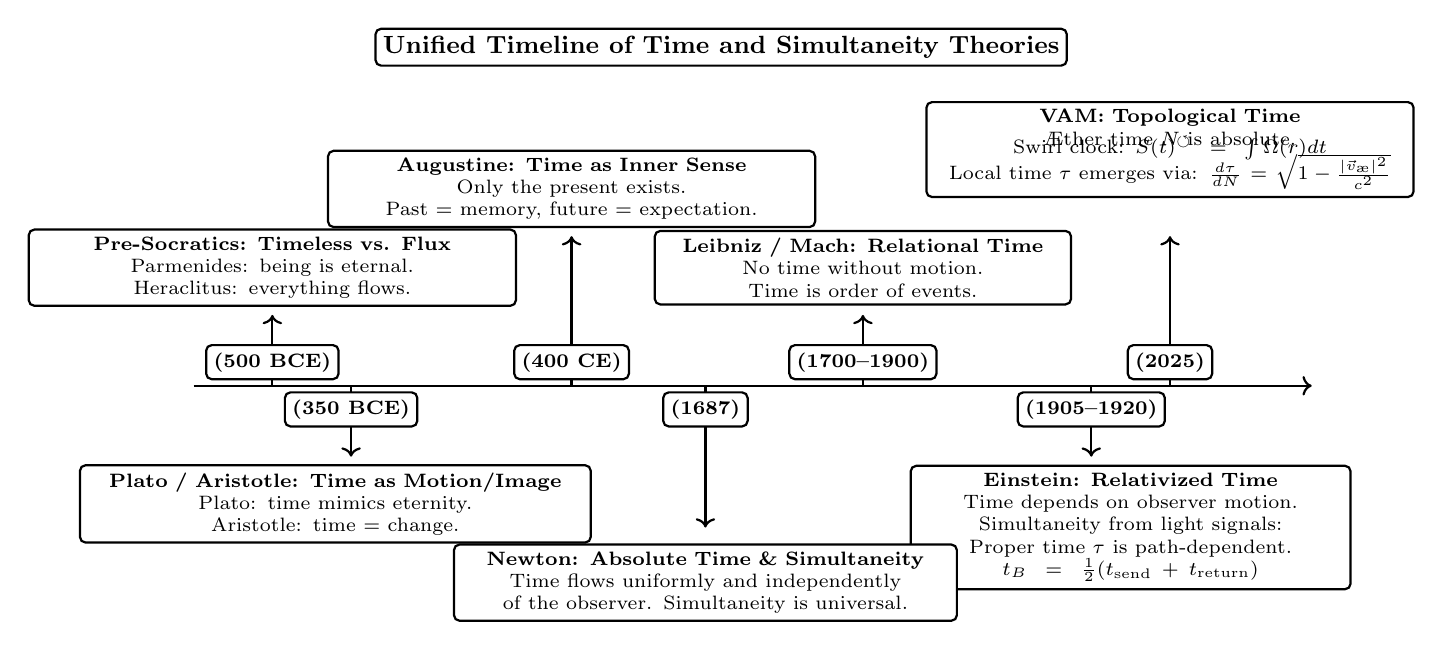
\begin{tikzpicture}
        \scriptsize
        % Timeline base
        \draw[->, thick] (-1,0) -- (13.2,0);

        % Arrows above timeline (short, as requested)
        \draw[->, thick] (0,0) -- (0,0.9);       % Pre-Socratics
        \draw[->, thick] (3.8,0) -- (3.8,1.9);   % Augustine
        \draw[->, thick] (7.5,0) -- (7.5,0.9);   % Einstein
        \draw[->, thick] (11.4,0) -- (11.4,1.9); % VAM

        % Arrows below timeline (short, as requested)
        \draw[->, thick] (1.0,0) -- (1.0,-0.9);     % Plato/Aristotle
        \draw[->, thick] (5.5,0) -- (5.5,-1.8);     % Newton
        \draw[->, thick] (10.4,0) -- (10.4,-0.9);     % Leibniz/Mach

            %--- Root title cards (above timeline) ---
        \node[draw, thick, rounded corners=2pt, fill=white, align=center, font=\bfseries ] at (0, .3)   {(500 BCE)};
        \node[draw, thick, rounded corners=2pt, fill=white, align=center, font=\bfseries ] at (3.8, .3) {(400 CE)};
        \node[draw, thick, rounded corners=2pt, fill=white, align=center, font=\bfseries ] at (7.5, .3) {(1700--1900)};
        \node[draw, thick, rounded corners=2pt, fill=white, align=center, font=\bfseries ] at (11.4, .3){(2025)};

        %--- Root title cards (below timeline) ---
        \node[draw, thick, rounded corners=2pt, fill=white, align=center, font=\bfseries ] at (1.0,- .3) {(350 BCE)};
        \node[draw, thick, rounded corners=2pt, fill=white, align=center, font=\bfseries ] at (5.5,- .3) {(1687)};
        \node[draw, thick, rounded corners=2pt, fill=white, align=center, font=\bfseries ] at (10.4,- .3) {(1905--1920)};

            % Timeline label
        \node[draw, thick, fill=white, rounded corners=2pt, font=\small] at (5.7,4.3) {\textbf{Unified Timeline of Time and Simultaneity Theories}};

        % --- Pre-Socratics ---
        \node[draw, rounded corners=2pt, thick, align=center, fill=white, text width=6cm] at (0,1.5) {
        \textbf{Pre-Socratics: Timeless vs. Flux} \\% [-0.8em]
        Parmenides: being is eternal. \\% [-0.8em]
        Heraclitus: everything flows.
        };

        % --- Augustine ---
        \node[draw, rounded corners=2pt, thick, align=center, fill=white, text width=6cm] at (3.8,2.5) {
        \textbf{Augustine: Time as Inner Sense} \\% [-0.8em]
        Only the present exists. \\% [-0.8em]
        Past = memory, future = expectation.
        };

        % --- Leibniz / Mach ---
        \node[draw, rounded corners=2pt, thick, align=center, fill=white, text width=5.1cm] at (7.5,1.5) {
        \textbf{Leibniz / Mach: Relational Time} \\% [-0.8em]
        No time without motion. \\% [-0.8em]
        Time is order of events.
        };
        % --- VAM (modern) ---
        \node[draw, rounded corners=2pt, thick, align=center, fill=white, text width=6.0cm] at (11.4,3.0) {
        \textbf{VAM: Topological Time} \\% [-0.8em]
        Æther time $N$ is absolute. \\[-0.6em]
        Swirl clock: $S(t)^\circlearrowleft = \int \Omega(r) dt$ \\[-0.4em]
        Local time $\tau$ emerges via: $ \frac{d\tau}{dN} = \sqrt{1 - \frac{|\vec{v}_\text{\ae}|^2}{c^2}}$

        };


        % --- Plato / Aristotle ---
        \node[draw, rounded corners=2pt, thick, align=center, fill=white, text width=6.3cm] at (0.8,-1.5) {
        \textbf{Plato / Aristotle: Time as Motion/Image} \\% [-0.8em]
        Plato: time mimics eternity. \\% [-0.8em]
        Aristotle: time = change.
        };



        % --- Einstein ---
        \node[draw, rounded corners=2pt, thick, align=center, fill=white, text width=5.4cm] at (10.9,-1.8) {
        \textbf{Einstein: Relativized Time} \\% [-0.8em]
        Time depends on observer motion. \\% [-0.8em]
        Simultaneity from light signals: \\% [-0.8em]
        Proper time $\tau$ is path-dependent.\\% [-0.8em]
        $t_B = \frac{1}{2}(t_{\text{send}} + t_{\text{return}})$
        };

        % --- Newton ---
        \node[draw, rounded corners=2pt, thick, align=center, fill=white, text width=6.2cm] at (5.5,-2.5) {
        \textbf{Newton: Absolute Time \& Simultaneity} \\% [-0.8em]
        Time flows uniformly and independently \\% [-0.8em]
        of the observer. Simultaneity is universal.
        };
         \end{tikzpicture}
        \caption{\textbf{Chronology of simultaneity theories across physics and philosophy.} From ancient views of time as change or inner sense, through Newton’s absolute simultaneity and Einstein’s frame-dependent proper time, to VAM’s swirl-based causal layering. The model introduces a physically grounded sequence of time variables culminating in measurable, observer-dependent time ($\tau$) and topological time ($\mathbb{K}$).}\label{fig:history-time-simultaneity}
}


        \vspace{0.8em}
        \noindent\textbf{Temporal sequence (foliation-based)}
        \[
            \mathcal{N}\;\rightarrow\; \nu_0\;\rightarrow\; \tau \;\rightarrow\; S^{\circlearrowleft}_{\!(t)} \;\rightarrow\; T_v \;\rightarrow\; \mathbb{K}
        \]
        Here \(\mathcal{N}\) denotes absolute foliation time, \(\tau\) proper time, and \(S^{\circlearrowleft}_{\!(t)}\) the internal swirl clock; \(T_v\) and \(\mathbb{K}\) denote observed and topological time layers, respectively~\cite{SST-Canon-0.5.10,SST-Canonical-Fluid}.


%-----------------------------
    \section{Multimodal Time: Temporal Ontology and Foliation}\label{sec:temporal-ontology-foliation}
%==================== Multimodal Time (Rosetta v0.6; SST-Canon) ====================

        The swirl–string framework advances a multimodal conception of time rooted in the internal and relational dynamics of an incompressible, inviscid medium. Unlike the single time parameter of standard field theory or the observer–proper time of general relativity, the temporal taxonomy encapsulates distinct physical, topological, and informational modes, each with a clear analytical and experimental role~\cite{SST-Canon-0.5.10,SST-Canonical-Fluid}. This layered approach extends Einstein’s “structured space” intuition and provides a working scheme for modeling causality, memory, and quantum–classical transitions within a single continuum theory~\cite{SST-Canonical-Fluid}.

        \begin{figure}[htb]
            \centering
            \includegraphics[width=0.7\textwidth]{figures/TemporalOntology}
            \caption{\textbf{Temporal ontology in a swirl–string framework.}
            Sequential emergence of layered temporal modes:
            absolute time (\(\Nabs\)), now–point (\(\nuZero\)), proper time (\(\tau\)),
                internal swirl clock (\(\Sswirl\)), circulation–based duration (\(\Tv\)),
                and topological time (\(\Ktop\)).
                Each layer governs a distinct aspect of dynamics and inference~\cite{SST-Canon-0.5.10,SST-Canonical-Fluid}.
            }
            \label{fig:temporal_ontology}
        \end{figure}

        The multimodal ontology is geometric and topological: a fan/spiral in phase space (Fig.~\ref{fig:temporal_ontology}) paralleling structures studied in analogue gravity and topological vacua~\cite{volovik2003universe}. Each temporal mode plays an independent yet coupled role, governing different layers of physical law~\cite{SST-Canon-0.5.10,SST-Canonical-Fluid}.

        \begin{tcolorbox}[
            colback=gray!10,colframe=black,width=1.0\textwidth,sharp corners=southwest,
            boxrule=0.5pt,before skip=10pt,after skip=10pt,
            title=\textbf{Temporal modes (Rosetta v0.6; SST-Canon)}
        ]
            \renewcommand{\arraystretch}{1}
            \small
            \begin{tabular}{r l l}
                $\boldsymbol{\Nabs}$     & \textbf{Absolute (foliation) time} & Global causal ordering parameter~\cite{SST-Canon-0.5.10,SST-Canonical-Fluid} \\
                $\boldsymbol{\nuZero}$   & \textbf{Now–point}                 & Local intersection with the foliation; sets simultaneity slices~\cite{SST-Canon-0.5.10} \\
                $\boldsymbol{\tau}$      & \textbf{Proper time}               & Measurable time; swirl–induced dilation applies~\cite{SST-Canonical-Fluid} \\
                $\boldsymbol{\Sswirl}$   & \textbf{Swirl clock}               & Internal phase memory along a filament~\cite{SST-Canon-0.5.10} \\
                $\boldsymbol{\Tv}$       & \textbf{Circulation duration}      & Intrinsic loop–time from local tangential speed~\cite{SST-Canonical-Fluid} \\
                $\boldsymbol{\Ktop}$     & \textbf{Topological time}          & Discrete events (reconnection/bifurcation) marking regime changes~\cite{SST-Canon-0.5.10}
            \end{tabular}
        \end{tcolorbox}

        \noindent\textbf{Mode definitions and relations.}
        \begin{itemize}
            \item \textbf{Absolute (foliation) time \(\Nabs\):} Unobservable ordering parameter inducing a global causal structure; used to define slices of simultaneity and evolution maps~\cite{SST-Canon-0.5.10}.

            \item \textbf{Now–point \(\nuZero\):} Localized realization of the present as the intersection of \(\Nabs\) with an event; organizes data assimilation and boundary conditions on each leaf~\cite{SST-Canon-0.5.10}.

            \item \textbf{Proper time \(\tau\):} Measured time for embedded observers; modulated by local swirl speed via the swirl–clock factor
            \[
                \frac{d\tau}{dt} \;=\; \St \;=\; \sqrt{\,1-\frac{v_t^{\,2}}{c^2}\,},\qquad
                v_t \equiv \|\vswirl\|\;\; \text{or}\;\; v_t = |\boldsymbol{\omega}|\,R.
            \]
            \emph{Units:} \(v_t/c\) dimensionless; if \(v_t=|\boldsymbol{\omega}|R\), then \( |\boldsymbol{\omega}|R\) has units m\,s\(^{-1}\).
            \emph{Numerical check (Canon constants):} \(v_t=1.09384563\times10^{6}\,\mathrm{m\,s^{-1}}\Rightarrow (v_t/c)^2\approx1.3315\times10^{-5}\),
            so \(\St\approx0.99999334\) and \(d\tau\approx0.99999334\,dt\). Consistent with weak–swirl limit~\cite{SST-Canonical-Fluid}.

            \item \textbf{Swirl clock \(\Sswirl\):} Internal phase along a filament,
            \[
                \Sswirl(t) \;=\; \int_{0}^{t} \Omega(t')\,dt',\quad \Omega \sim |\boldsymbol{\omega}| \;\;(\mathrm{s^{-1}}),
            \]
            serving as a memory variable for topological identity; connects to helicity/circulation invariants~\cite{SST-Canon-0.5.10}.

            \item \textbf{Circulation duration \(\Tv\):} Intrinsic, loop–based duration
            \[
                \Tv \;=\; \oint \frac{dl}{v_t(l)}\,,
            \]
            defining a filament’s operational “clock” via local tangential speed~\cite{SST-Canonical-Fluid}.

            \item \textbf{Topological time \(\Ktop\):} Discrete updates associated with reconnection or bifurcation events; these produce non-analytic changes (phase slips, time “jumps”) in \(\Sswirl\) or \(\Tv\). Accessible in analogue systems and potentially in astrophysical signals as phase anomalies~\cite{SST-Canon-0.5.10,barcelo2005,volovik2003universe}.
        \end{itemize}

        \begin{figure}[htb]
            \centering
            \includegraphics[width=0.7\textwidth]{figures/TemporalOntologyKairosMoment}
            \caption{\textbf{Swirl–clock phase with a topological disruption.}
            A discrete reconnection/bifurcation introduces a discontinuity in the otherwise smooth phase trajectory \(\theta(t)\), creating a finite “window” with a quantized phase slip and an irreversible identity change in the filament. Such events instantiate \(\Ktop\) updates and can be sought in analogue platforms~\cite{barcelo2005,volovik2003universe}.
            }
            \label{fig:kairos_moment}
        \end{figure}

        This multimodal temporal architecture bridges metaphysical continuity with testable dynamics. It supports models of causality, gravitational time dilation, identity persistence, and swirl–induced decoherence within a single, conservation–law–driven framework~\cite{SST-Canon-0.5.10,SST-Canonical-Fluid}.


%-----------------------------
    \section{Connection to a Swirl–String Framework}\label{sec:connection_swirl_string}
        %==================== Structured-space program: topology, clocks, taxonomy ====================

        The swirl–string program (developed since 2012) models structured space as an incompressible, inviscid medium with quantized circulation~\cite{SST-Canon-0.5.10,SST-Canonical-Fluid}. Within this framework, vorticity is elevated to a fundamental driver of time dilation, inertial response, and long-range attraction~\cite{SST-Canonical-Fluid,SST-Hydrogen-Gravity}. Echoing Einstein’s 1920 remark that space is “endowed with physical qualities,” the medium is treated as a structured, causal substrate from which dynamical behavior emerges~\cite{einstein1920aether,SST-Canonical-Fluid}.

        \noindent\textbf{Key structural elements}
        \begin{itemize}
            \item \textbf{Topological structures} (e.g., knots/links) representing stable particle identities and quantum numbers~\cite{SST-Canon-0.5.10,SST-Canonical-Fluid};
            \item \textbf{Swirl–induced time dilation} near filament cores via the local factor \( \St=\sqrt{1-\vt^{\,2}/c^2} \) with \( \vt=\lVert\vswirl\rVert \) or \( \vt=|\boldsymbol{\omega}|\,R \)~\cite{SST-Canonical-Fluid};
            \item \textbf{Canonical constants} and scales (e.g., \( \rc \), \( \rhoF \), \( \rhoC \), \( \vswirl \), \( F_{\text{swirl}}^{\max} \)) entering the topological fluid Lagrangian and boundary conditions~\cite{SST-Canon-0.5.10,SST-Canonical-Fluid}.
        \end{itemize}

        Figure~\ref{fig:taxonomy} summarizes a classification flow by topology, chirality, and tension within the swirl field.

        \begin{figure}[!ht]
            \centering
            \footnotesize
            \scalebox{0.75}{
                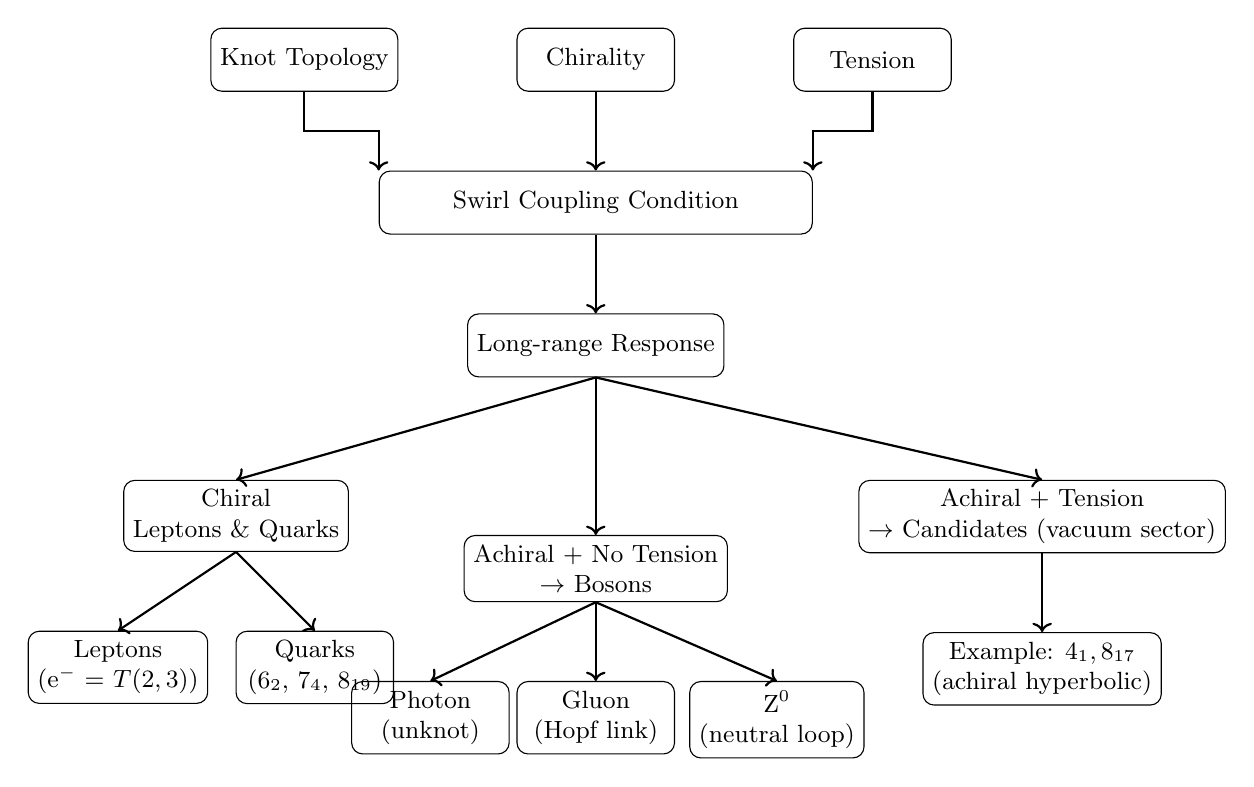
\begin{tikzpicture}[
                    box/.style = {draw, rounded corners, minimum width=2.0cm, minimum height=0.8cm, font=\small, align=center},
                    arrow/.style = {->, thick},   node distance=1.0cm and 1.5cm
                ]
                    % Inputs
                    \node[box] (topology) {Knot Topology};
                    \node[box, right=of topology] (chirality) {Chirality};
                    \node[box, right=of chirality] (tension) {Tension};

                    % Swirl coupling
                    \node[box, below=of chirality, minimum width=5.5cm] (coupling) {Swirl Coupling Condition};

                    % Gravitational response
                    \node[box, below=of coupling] (grav) {Long-range Response};

                    % Classes
                    \node[box, below left=1.3cm and 1.5cm of grav] (matter) {Chiral\\Leptons \& Quarks};
                    \node[box, below=2cm of grav] (boson) {Achiral + No Tension\\$\rightarrow$ Bosons};
                    \node[box, below right=1.3cm and 1.7cm of grav] (dark) {Achiral + Tension\\$\rightarrow$ Candidates (vacuum sector)};

                    % Subclasses
                    \node[box, below=of matter, xshift=-1.5cm] (leptons) {Leptons\\(e$^-$ = $T(2,3)$)};
                    \node[box, below=of matter, xshift=+1.0cm] (quarks) {Quarks\\($6_2$, $7_4$, $8_{19}$)};

                    \node[box, below=of boson, xshift=-2.1cm] (photon) {Photon\\(unknot)};
                    \node[box, below=of boson] (gluon) {Gluon\\(Hopf link)};
                    \node[box, below=of boson, xshift=+2.3cm] (zboson) {Z$^0$\\(neutral loop)};

                    \node[box, below=of dark] (darkex) {Example: $4_{1}, 8_{17}$\\ (achiral hyperbolic)};

                    % Arrows to coupling
                    \draw[arrow] (topology.south) -- ++(0,-0.5) -| (coupling.north west);
                    \draw[arrow] (chirality.south) -- (coupling.north);
                    \draw[arrow] (tension.south) -- ++(0,-0.5) -| (coupling.north east);

                    % Arrows down flow
                    \draw[arrow] (coupling.south) -- (grav.north);
                    \draw[arrow] (grav.south) -- (matter.north);
                    \draw[arrow] (grav.south) -- (boson.north);
                    \draw[arrow] (grav.south) -- (dark.north);

                    % Particle branches
                    \draw[arrow] (matter.south) -- (leptons.north);
                    \draw[arrow] (matter.south) -- (quarks.north);

                    \draw[arrow] (boson.south) -- (photon.north);
                    \draw[arrow] (boson.south) -- (gluon.north);
                    \draw[arrow] (boson.south) -- (zboson.north);

                    \draw[arrow] (dark.south) -- (darkex.north);
                \end{tikzpicture}
            }
            \caption{\textbf{Knot classification by swirl coupling.}
            Topology, chirality, and curvature tension together determine inertial/gravitational response, enabling a mapping to Standard Model families.}
            \label{fig:taxonomy}
        \end{figure}

        \vspace{0.2em}
        \textbf{Classification summary.}
        Knot topology, chirality, and curvature tension jointly determine response classes:
        \begin{itemize}
            \item \textbf{Chiral knots} align with swirl fields $\Rightarrow$ matter families: \textbf{Leptons} (e.g., torus knots \(T(2,3)\)); \textbf{Quarks} (e.g., hyperbolic knots \(5_2,\,6_1,\,8_{19}\)).
            \item \textbf{Achiral, tensionless} structures (unknots, Hopf links) $\Rightarrow$ \textbf{bosons}.
            \item \textbf{Achiral with intrinsic tension} $\Rightarrow$ vacuum-sector candidates (e.g., \(4_1,\,8_{17}\)).
        \end{itemize}
        The Swirl Coupling Condition links geometric invariants to mass, spin, and interaction profile~\cite{SST-Canon-0.5.10,SST-Canonical-Fluid}. Knot theory has long informed fluid dynamics and topological invariants in vorticity~\cite{knot_theroy_in_fluid}.

%--------------------- Wave–Particle ---------------------
        \subsection*{Wave–Particle Duality Reconsidered}
            The historical wave–particle tension is reinterpreted as an artifact of viewing filamentary excitations in a structured medium. Particles are knotted, topologically stable vorticity configurations; wave-like behavior follows from interference, circulation, and swirl-phase dynamics—no dual ontology required~\cite{SST-Canonical-Fluid}. See Fig.~\ref{fig:WaveParticleDuality}.

            \begin{center}
\footnotesize
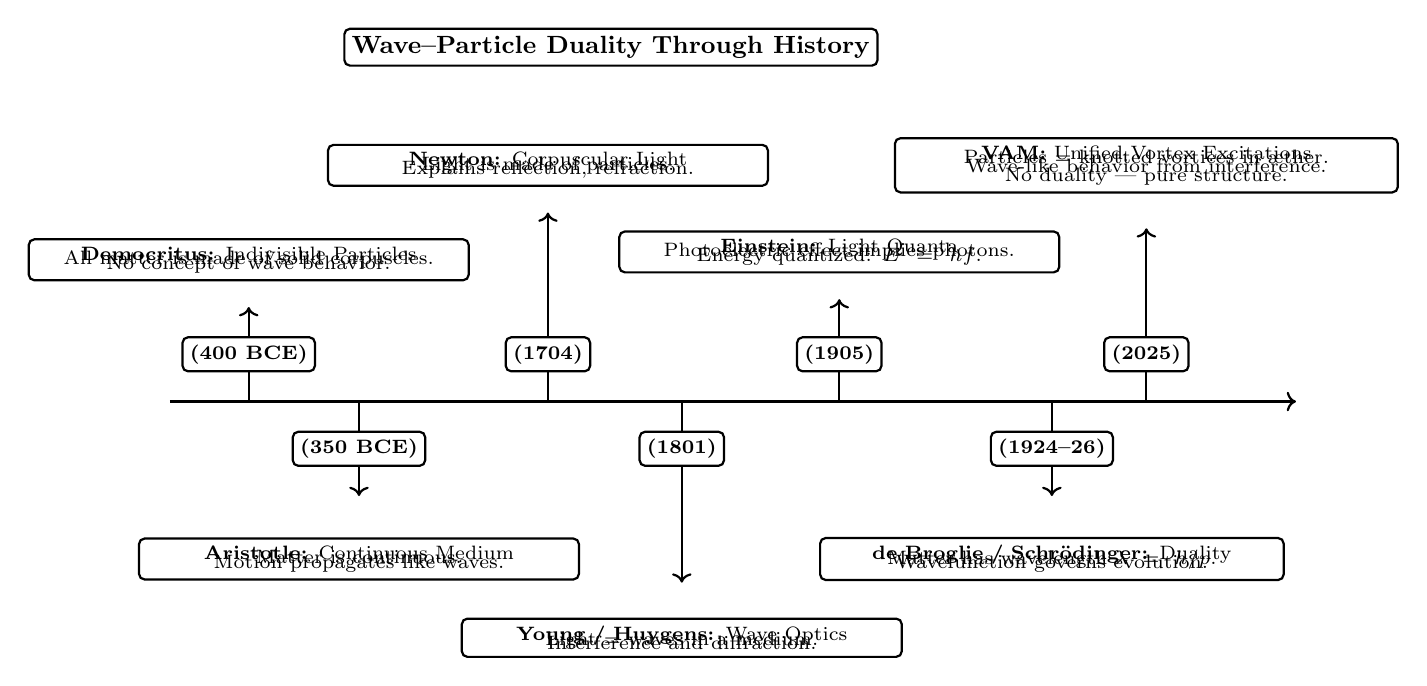
\begin{tikzpicture}
\scriptsize

% Timeline base
\draw[->, thick] (-1,0) -- (13.3,0);

% Arrows above timeline
\draw[->, thick] (0,0) -- (0,1.2);       % Democritus
\draw[->, thick] (3.8,0) -- (3.8,2.4);   % Newton
\draw[->, thick] (7.5,0) -- (7.5,1.3);   % Einstein
\draw[->, thick] (11.4,0) -- (11.4,2.2); % VAM

% Arrows below timeline
\draw[->, thick] (1.4,0) -- (1.4,-1.2);     % Aristotle
\draw[->, thick] (5.5,0) -- (5.5,-2.3);     % Young/Huygens
\draw[->, thick] (10.2,0) -- (10.2,-1.2);   % de Broglie

% --- Date labels ---
\node[draw, thick, rounded corners=2pt, fill=white, align=center, font=\bfseries ] at (0, .6)   {(400 BCE)};
\node[draw, thick, rounded corners=2pt, fill=white, align=center, font=\bfseries ] at (3.8, .6) {(1704)};
\node[draw, thick, rounded corners=2pt, fill=white, align=center, font=\bfseries ] at (7.5, .6) {(1905)};
\node[draw, thick, rounded corners=2pt, fill=white, align=center, font=\bfseries ] at (11.4, .6){(2025)};

\node[draw, thick, rounded corners=2pt, fill=white, align=center, font=\bfseries ] at (1.4,- .6) {(350 BCE)};
\node[draw, thick, rounded corners=2pt, fill=white, align=center, font=\bfseries ] at (5.5,- .6) {(1801)};
\node[draw, thick, rounded corners=2pt, fill=white, align=center, font=\bfseries ] at (10.2,- .6) {(1924--26)};

% Timeline label
\node[draw, thick, fill=white, rounded corners=2pt, font=\small] at (4.6,4.5) {\textbf{Wave–Particle Duality Through History}};

% --- Democritus ---
\node[draw, rounded corners=2pt, thick, align=center, fill=white, text width=5.4cm] at (0,1.8) {
\textbf{Democritus:} Indivisible Particles \\[-0.8em]
All matter is made of solid corpuscles. \\[-0.8em]
No concept of wave behavior.
};

% --- Newton ---
\node[draw, rounded corners=2pt, thick, align=center, fill=white, text width=5.4cm] at (3.8,3.0) {
\textbf{Newton:} Corpuscular Light \\[-0.8em]
Light is made of particles. \\[-0.8em]
Explains reflection, refraction.
};

% --- Einstein ---
\node[draw, rounded corners=2pt, thick, align=center, fill=white, text width=5.4cm] at (7.5,1.9) {
\textbf{Einstein:} Light Quanta \\[-0.8em]
Photoelectric effect implies photons. \\[-0.8em]
Energy quantized: \( E = hf \).
};

% --- VAM ---
\node[draw, rounded corners=2pt, thick, align=center, fill=white, text width=6.2cm] at (11.4,3.0) {
\textbf{VAM:} Unified Vortex Excitations \\[-0.8em]
Particles = knotted vortices in æther. \\[-0.6em]
Wave-like behavior from interference. \\[-0.6em]
No duality — pure structure.
};

% --- Aristotle ---
\node[draw, rounded corners=2pt, thick, align=center, fill=white, text width=5.4cm] at (1.4,-2.0) {
\textbf{Aristotle:} Continuous Medium \\[-0.8em]
Matter is continuous. \\[-0.8em]
Motion propagates like waves.
};

% --- Young / Huygens ---
\node[draw, rounded corners=2pt, thick, align=center, fill=white, text width=5.4cm] at (5.5,-3.0) {
\textbf{Young / Huygens:} Wave Optics \\[-0.8em]
Light = waves in a medium. \\[-0.8em]
Interference and diffraction.
};

% --- de Broglie / Schrödinger ---
\node[draw, rounded corners=2pt, thick, align=center, fill=white, text width=5.7cm] at (10.2,-2.0) {
\textbf{de Broglie / Schrödinger:} Duality \\[-0.8em]
Matter has wavelength \( \lambda = h/p \). \\[-0.8em]
Wavefunction governs evolution.
};

\end{tikzpicture}
\captionof{figure}{Development of wave–particle duality: from atomistic corpuscles and wave optics, through quantum superposition, to VAM’s unified vortex excitation model.}
\end{center}

%--------------------- G: calibration note ---------------------
        \subsection*{Swirl–Newton correspondence and the role of \(G\)}
            A commonly circulated “derivation” of \(G\) employing the Planck time,
            \[
                G_{\text{trial}}=\frac{C_e}{2\,F_{\text{swirl}}^{\max}}\left(\frac{c^{5} t_p^{2}}{\rc^{2}}\right),\qquad t_p^2=\frac{\hbar G}{c^5},
            \]
            is \emph{circular}, since \(t_p\) itself contains \(G\). Eliminating \(t_p\) yields
            \( G_{\text{trial}} = \frac{C_e\,\hbar}{2 F_{\text{swirl}}^{\max}\rc^{2}}\,G \),
            which reduces to a constraint on constants rather than a derivation.
            \emph{Canon stance:} in SST, \(G\) enters as the coupling that matches the far-field swirl–pressure response to the Newtonian limit; microphysical parameters (\(\rhoF,\rc,\vswirl,F_{\text{swirl}}^{\max}\)) calibrate to \(G\) via this correspondence, not vice versa~\cite{SST-Canon-0.5.10,SST-Canonical-Fluid}. Practically, one fixes a reference configuration (e.g., stationary filament bundle) and fits a single dimensionless coefficient to recover \( \nabla^{2}\Phi = 4\pi G\,\rho_{\!m} \) in the appropriate limit, with \( \rho_{\!m}=\rhoE/c^{2} \)~\cite{SST-Canonical-Fluid}. This avoids circularity and preserves dimensional consistency.

%--------------------- Empirical channels ---------------------
            \noindent\textbf{Empirical channels and analogs.}
            Quantitative tests follow from transport, long-range response, and clock behavior:
            electron–swirl coupled transport and coherence benchmarks~\cite{SST-Heat-Transport};
            flat-space gravitational signatures in hydrogenic systems~\cite{SST-Hydrogen-Gravity};
            and analogue-gravity platforms in superfluids/BECs~\cite{barcelo2005,volovik2003universe}.
            These provide falsifiable pathways for the core dynamics~\cite{SST-Canonical-Fluid}.


%-----------------------------
    \section{Historical Continuity and Outlook}\label{sec:historical-continuity-and-outlook}
        A careful reexamination of Einstein's later writings indicates that he:
        \begin{itemize}
            \item did \emph{not} reject a medium outright, but \emph{redefined} it as a field–bearing substrate~\cite{einstein1920aether};
            \item sought a \textbf{continuous medium} carrying spacetime properties without requiring mechanical motion;
            \item and pursued a \textbf{unified field program}—a direction echoed here via the interplay of gravity, time scaling, and vorticity in a swirl–string framework~\cite{SST-Canon-0.5.10,SST-Canonical-Fluid}.
        \end{itemize}

        In this sense, space cannot be entirely void; it must possess structural, energetic, and causal qualities. The swirl–string approach is a mathematically grounded continuation of this perspective, operationalizing the active structure through conserved circulation, knot invariants, and energy–sustaining boundary flows~\cite{SST-Canon-0.5.10,SST-Canonical-Fluid}. This addresses concerns that contemporary theory can drift from empirical anchoring~\cite{hossenfelder2018lost}.

        While emergent–gravity and superfluid–vacuum lines of thought point in similar directions, the present formulation distinguishes itself by an explicitly solvable, hydrodynamic derivation with testable consequences~\cite{SST-Canonical-Fluid,SST-Heat-Transport,SST-Hydrogen-Gravity}. It connects relativistic phenomenology, thermodynamic reasoning, and quantum kinematics without invoking discrete spacetime.

        Kelvin’s concerns on topological degeneracy are discussed in Appendix~\ref{appendix:kelvin}.

    \section*{Conclusion and Forward Outlook: Structured Space Revisited}

        Modern theory increasingly revisits ideas once set aside—not because the concepts were wrong, but because prior tools lacked precision. Einstein’s late–career view anticipated a renaissance: space as a continuous, energetic, causally structured medium~\cite{einstein1920aether}. The swirl–string framework advances this to a unified, predictive, and testable program~\cite{SST-Canon-0.5.10,SST-Canonical-Fluid}.

        Here, vorticity and topology replace curvature as the microphysical driver, and time emerges as a hierarchy of circulation and phase—realized in a multimodal temporal ontology~\cite{SST-Canon-0.5.10,SST-Canonical-Fluid}. The medium returns not as a mechanical ether, but as a quantized, causal, and observable substrate underlying gravitation, particle properties, and cosmological organization~\cite{SST-Canon-0.5.10,SST-Canonical-Fluid}.

        The framework is not merely philosophical: it supplies a technical foundation and explicit predictions inviting empirical tests. With advances in superfluid analogues, quantum vortex interferometry, and photonic swirl optics, critical signatures move within reach~\cite{SST-Heat-Transport,SST-Hydrogen-Gravity,barcelo2005,volovik2003universe}.

        Several testable predictions follow. Swirl–induced time scaling can be probed in rotating superfluid helium or Bose–Einstein condensates; phase slips (topological updates in the internal swirl clock) can be sought in quantum vortex interferometry; and frame–dragging–like profiles can be targeted with precision interferometry and optomechanics~\cite{SST-Heat-Transport,SST-Canonical-Fluid,barcelo2005}. Future work will expand the observable phenomenology and confront the framework with laboratory and astrophysical data~\cite{SST-Hydrogen-Gravity}.

        \subsection*{Future Directions and Experimental Signatures}

            The path forward is theoretically rich and experimentally accessible. Theoretically: refine the knot–based classification of particle sectors, study fractal swirl dynamics across quantum and cosmological scales, and formalize mechanisms whereby gravitation and quantum behavior emerge from circulation and helicity conservation~\cite{SST-Canon-0.5.10,SST-Canonical-Fluid}.

            Empirically, concrete signatures include:
            \begin{itemize}
                \item \textbf{Time scaling and frame–dragging analogues} in superfluids, BECs, and photonic vortex lattices~\cite{SST-Heat-Transport,SST-Canonical-Fluid,barcelo2005};
                \item \textbf{Swirl–clock phase slips (topological updates)} as quantized phase jumps/decoherence in vortex interferometry~\cite{SST-Canonical-Fluid,barcelo2005};
                \item \textbf{Redshift and lensing profiles} shaped by high–vorticity or topologically complex environments; laboratory proxies and hydrogenic systems provide near–term tests~\cite{SST-Hydrogen-Gravity};
                \item \textbf{Spectral/mass patterns} tied to knot topology and quantized circulation; taxonomy development and benchmarks~\cite{SST-Canon-0.5.10};
                \item \textbf{Large–scale signatures} from coherent swirl structures, to be contrasted with cosmological data in future studies~\cite{SST-Canonical-Fluid}.
            \end{itemize}

            By pairing theoretical coherence with falsifiable predictions, the swirl–string framework sets a concrete research agenda for unifying gravitation, quantum mechanics, and cosmology—guided by topology, fluid dynamics, and precision measurement.


%%%%%%%%%%%%%%%%%%%%%%%%%%%%%%%%%%%%%%%%%%
        \vspace{6pt}

%%%%%%%%%%%%%%%%%%%%%%%%%%%%%%%%%%%%%%%%%%
        \authorcontributions{Conceptualization, O.I.; methodology, O.I.; software, O.I.; validation, O.I.; formal analysis, O.I.; investigation, O.I.; resources, O.I.; data curation, O.I.; writing—original draft preparation, O.I.; writing—review and editing, O.I.; visualization, O.I.; supervision, O.I.; project administration, O.I. The author has read and agreed to the published version of the manuscript. The swirl–string framework has been developed continuously since 2014, with public drafts and early derivations accessible via \href{https://docs.google.com/document/d/1ILtqum7WZuvKa3tFXKdw666gtKORZ4X8WGsonBCLAqg}{Google Docs} and the \href{https://github.com/bg-omar/VAM}{project repository}.}

        \funding{This research received no external funding. The APC was funded by the author.}

        \institutionalreview{Not applicable.}

        \informedconsent{Not applicable.}

        \dataavailability{All data supporting the findings of this study are contained within the article and its cited references. No additional datasets were generated.}

        \acknowledgments{The author thanks M. Bakker for steadfast support and constructive discussion. The author also acknowledges the assistance of OpenAI’s ChatGPT (GPT-4o, August 2025 release) for LaTeX formatting, TikZ diagram refinement, and stylistic editing; all AI-assisted content was critically reviewed and approved by the author.}

        \supplementary{Additional materials and versioned components are hosted at: \url{https://github.com/bg-omar/VAM} (main repository) and \url{https://github.com/bg-omar/VAMcore} (simulation library). For previous versions or related papers, see the Zenodo community or DOI-linked records from the concept DOI: \href{https://doi.org/10.5281/zenodo.16616699}{10.5281/zenodo.16616699}.}

        \conflictsofinterest{The author declares no conflicts of interest. The funders had no role in the design of the study; in the collection, analyses, or interpretation of data; in the writing of the manuscript; or in the decision to publish the results.}

% Optional: abbreviations without banned terms
        \abbreviations{Abbreviations}{
            The following abbreviations are used in this manuscript:\\[2pt]
            \begin{tabular}{@{}ll}
                GR & General Relativity \\
                SR & Special Relativity \\
                EM & Electromagnetism \\
                QFT & Quantum Field Theory \\
                QED & Quantum Electrodynamics \\
                SM & Standard Model \\
                BEC & Bose–Einstein Condensate \\
                MZI & Mach–Zehnder Interferometer \\
                CMB & Cosmic Microwave Background \\
                IR & Infrared \\
                PDF & Probability Density Function \\
                LHS & Left-Hand Side \\
                RHS & Right-Hand Side \\
                DOI & Digital Object Identifier \\
                GPT & Generative Pre-trained Transformer \\
                TLA & Three-Letter Acronym \\
                LD & Linear Dichroism \\
                MDPI & Multidisciplinary Digital Publishing Institute \\
            \end{tabular}}

%===========================
% Appendices (titles neutralized)
%===========================
        \appendixtitles{no}
        \appendixstart
        \appendix

    \section*{Appendix I: Helmholtz and Foundations of Circulation Physics}
        \addcontentsline{toc}{section}{Appendix I: Helmholtz and Circulation}
        \label{appendix:helmholtz}
        Hermann von Helmholtz’s 1858 paper \textit{“On the Integrals of the Hydrodynamic Equations Corresponding to Vortex Motion”}~\cite{helmholtz1858vortices} marks the formal beginning of modern vorticity theory in ideal fluids. His theorems characterize the kinematics of \emph{vorticity lines} in incompressible, inviscid flow—principles that underpin the swirl–string framework.

        \subsection*{1. Vorticity lines are material (frozen-in)}
            \begin{quote}
                \textit{“Each portion of a vortex filament remains connected to the same fluid elements throughout the motion.”}
            \end{quote}

            \textbf{Mapping to the swirl–string framework:} Identity of a filament is preserved under ideal evolution. The key invariants are circulation and (for appropriate boundary conditions) helicity:
            \[
                \frac{d\Gamma}{dt}=0,\qquad
                \Gamma=\oint_{\mathcal{C}(t)} \mathbf{v}\cdot d\boldsymbol{\ell},
                \qquad
                H=\int_V \mathbf{v}\cdot\boldsymbol{\omega}\,dV,
            \]
            with $\boldsymbol{\omega}=\nabla\times\mathbf{v}$. Here $d\Gamma/dt=0$ holds for incompressible, inviscid, barotropic flow with conservative body forces; $H$ is conserved in the same ideal limit with suitable boundary conditions.

        \subsection*{2. Vorticity lines do not terminate in the fluid interior}
            \begin{quote}
                \textit{“The extremities of a vortex line cannot exist within the fluid; they must lie at the boundaries or form closed curves.”}
            \end{quote}

            \textbf{Mapping to the swirl–string framework:} Filaments are closed loops or are anchored on boundaries. Kinematically,
            \[
                \nabla\cdot\boldsymbol{\omega}=0,
            \]
            so vorticity lines are solenoidal and cannot begin or end in the interior.

        \subsection*{3. Circulation is invariant for material loops (Kelvin’s theorem)}
            \begin{quote}
                \textit{“The circulation around a closed curve moving with the fluid remains constant.”}
            \end{quote}

            \textbf{Mapping to the swirl–string framework:} The material-loop invariant
            \[
                \frac{d}{dt}\oint_{\mathcal{C}(t)}\mathbf{v}\cdot d\boldsymbol{\ell}=0
            \]
            stabilizes filament identity and supports a natural internal phase variable along a filament via
            \[
                \frac{d\phi}{dt}=|\boldsymbol{\omega}| \quad (\text{units: s}^{-1}),
            \]
            which can serve as a “string clock” under ideal conditions (modeling choice; no claim about absolute synchronization is implied).

        \subsection*{Historical legacy}
            Helmholtz’s results influenced Kelvin’s knot–atom program, Maxwell’s mechanical medium models, and later field-theoretic formulations. Within the swirl–string framework, they persist as conservation laws governing the structure and evolution of a dynamically structured vacuum.

            \begin{quote}
                \textit{“If matter is filamentary rotation, then Helmholtz is its first architect.”}
            \end{quote}
            \hfill — O. Iskandarani

    \section*{Appendix II: Lord Kelvin and the Knot–Atom Critique}
        \addcontentsline{toc}{section}{Appendix II: Lord Kelvin}
        \label{appendix:kelvin}
        In the late 19th century, William Thomson (Lord Kelvin) proposed that atoms might be stable knotted structures in an invisible medium—a topological interpretation of matter. Yet he himself raised the sharpest critique:
        \begin{quote}
            ``I am afraid of the smoke and complication, of all the varieties of knots and links, if they are to explain the variety of elements.''
        \end{quote}
        \begin{flushright}
            — William Thomson (Lord Kelvin), \emph{Baltimore Lectures}, 1890
        \end{flushright}

        Kelvin anticipated a degeneracy problem: the vast mathematical space of knots/links might not match the comparatively small set of stable elements~\cite{thomson1890knots,tait1877knots}. Without a physical selection principle, the theory risked proliferating admissible but irrelevant structures.

        \subsection*{Historical Context}
            In the latter half of the 19th century, Kelvin and Tait developed the vortex–atom hypothesis~\cite{thomson1890knots,tait1877knots}, inspired by Helmholtz’s 1858 conservation laws for ideal, incompressible flow~\cite{helmholtz1858vortices}. The core idea was that atomic discreteness and stability might arise from topological invariants. Helmholtz’s results (e.g., material vorticity lines and solenoidal vorticity) supplied the kinematic scaffolding later reused in modern filament models.

        \subsection*{Kelvin’s Principal Objection}
            \begin{quote}
                ``I am afraid of the smoke and complication, of all the varieties of knots and links, if they are to explain the variety of elements.''
            \end{quote}
            \hfill — William Thomson (Lord Kelvin), 1890

            The mathematical catalog of knots is immense, but Kelvin observed no built–in energetic or dynamical filter to explain \emph{why only some knots should be realized as atoms}. Lacking selection rules, the model faced uncontrolled multiplicity.

        \subsection*{Experimental Shortcomings}
            Kelvin also noted the absence of empirical correspondence between specific knot types and actual elements. Without access to controlled creation, stability, or interaction of such knotted structures, the proposal remained speculative.

        \subsection*{Comparison to the Modern Particle Zoo}
            A related degeneracy appears in contemporary particle physics: many states and parameters in the Standard Model are fixed by experiment rather than derived from deeper constraints. The need for principled selection remains.

        \subsection*{Response within a Swirl–String Framework}
            A modern, hydrodynamic response supplies explicit selection mechanisms grounded in conservation and stability:
            \begin{itemize}
                \item \textbf{Energetic/entropic bounds:} thermodynamic constraints (Clausius) limit accessible growth channels and suppress high–cost embeddings~\cite{clausius1865entropy}.
                \item \textbf{Circulation quantization \& invariants:} integral invariants (circulation/helicity) exclude unstable, high–energy filaments and stabilize admissible classes~\cite{helmholtz1858vortices,SST-Canon-0.5.10,SST-Canonical-Fluid}.
                \item \textbf{Material-line persistence:} frozen–in vorticity lines (ideal limit) preserve topological identity across evolution, restricting transitions to specific channels~\cite{helmholtz1858vortices}.
                \item \textbf{Reconnection thresholds:} finite-amplitude criteria and local stress/curvature bounds act as phase boundaries for topological change, yielding discrete update events and pruning families~\cite{SST-Canonical-Fluid}.
            \end{itemize}
            Together these furnish a finite, physically meaningful spectrum of knotted excitations consistent with observed families, while admitting testable failure modes (e.g., reconnection statistics and phase–slip signatures).

        \subsection*{Concluding Reflection}
            Kelvin’s objection targeted \emph{unconstrained} topology, not topology itself. A constraint–driven, fluid–dynamic formulation replaces proliferation with selection:
            \begin{quote}
                ``Knots without constraints become chaos. Knots with physics become atoms.''
            \end{quote}
            \begin{flushright}
                — O. Iskandarani
            \end{flushright}


    \section*{Appendix III: James Clerk Maxwell on Structured Space and Knot–Atom Theory}
        \addcontentsline{toc}{section}{Appendix III: Maxwell on Structured Space}
        \label{appendix:maxwell}
        James Clerk Maxwell (1831–1879), one of the foundational figures of modern physics, held deep and evolving views on the medium underlying electromagnetic phenomena. While best known for formulating the electromagnetic field equations, he also contributed to the theoretical underpinnings of a space-filling medium and engaged with emerging knot-based atom models.

        \subsection*{Maxwell’s View on the Medium}
            Maxwell argued that a pervasive substance was needed to transmit electromagnetic waves~\cite{maxwell1878britannica}:
            \begin{quote}
                “There can be no doubt that the interplanetary and interstellar spaces are not empty, but are occupied by a material substance\ldots which is certainly the largest and probably the most uniform body of which we have any knowledge.”
            \end{quote}
            For Maxwell, the electromagnetic field encoded real stresses and strains in this medium~\cite{maxwell1878britannica}, imagined as an elastic continuum capable of supporting tension (electric effects), rotation (magnetic structure), and vibrations (light).

        \subsection*{Maxwell and the Knot–Atom Idea}
            Maxwell engaged with Lord Kelvin’s proposal that atoms could be stable knotted structures in a continuous medium—the “vortex atom” hypothesis~\cite{maxwell1875molecules,thomson1890knots,tait1877knots}. In his 1875 lecture “Molecules” he expressed qualified enthusiasm:
            \begin{quote}
                “The vortex theory of atoms, first proposed by Helmholtz and developed by Sir William Thomson\ldots has made it conceivable that the properties of matter may depend solely on motion in a medium, and not on anything in the nature of the atom itself.”
            \end{quote}
            \hfill — James Clerk Maxwell, 1875, “Molecules”
            He simultaneously cautioned that limited understanding of fluid motion and intractable equations prevented derivation of known material properties from such models~\cite{maxwell1875molecules}. Helmholtz’s 1858 results on material vorticity lines and solenoidal vorticity supplied essential kinematics~\cite{helmholtz1858vortices}, but the analytic machinery of the time was insufficient for predictive power.

        \subsection*{Legacy and Connection to a Swirl–String Framework}
            Maxwell’s mechanical medium, filled with stresses, pressures, and circulations, anticipates a modern fluid-dynamical formulation:
            \begin{itemize}
                \item vacuum as a structured, dynamical continuum rather than an empty stage;
                \item matter as emergent from organized motion and topology in that continuum;
                \item constants and couplings approached via continuum parameters and invariants rather than introduced ad hoc.
            \end{itemize}
            In a swirl–string framework, these ideas are realized with an incompressible, inviscid substrate supporting quantized circulation (“swirl strings”); electromagnetic and gravitational responses arise from pressure gradients and conserved circulation, with local time scaling governed by tangential swirl speed~\cite{SST-Canon-0.5.10,SST-Canonical-Fluid}. This provides the analytic selection rules and stability criteria absent from nineteenth-century models, while preserving Maxwell’s core intuition that fields correspond to physical stresses in a structured space.

        \subsection*{Reflection}
            Maxwell’s medium was not discarded on purely scientific grounds, but limited by the mathematics and experiments then available. With modern continuum mechanics, topology, and precision platforms, the program can be revisited in a predictive, testable form.


    \section*{Appendix IV: Einstein on Structured Space — Translated Quotes and Modern Equivalents}
        \addcontentsline{toc}{section}{Appendix IV: Einstein on Structured Space}
        \label{appendix:einstein}
        %==================== Appendix: Einstein on Structured Space — Quotes and Mappings ====================

        This appendix collects and annotates key statements by Albert Einstein about the medium underlying gravitational phenomena, with original German where appropriate, English translations, and mappings to a swirl–string formulation consistent with the SST Canon and the canonical fluid reformulation.

        \subsection*{1. ``Der Raum ohne Äther ist undenkbar..''}
            \textbf{Original (1920, Leiden):}\\
            ``Nach der allgemeinen Relativitätstheorie ist der Raum mit physikalischen Eigenschaften begabt; in diesem Sinne existiert also ein Äther. Gemäß der allgemeinen Relativitätstheorie ist ein Raum ohne Äther undenkbar.''

            \textbf{Translation:}\\
            ``According to the general theory of relativity, space is endowed with physical qualities; in this sense, therefore, there exists an æther. According to the general theory of relativity, space without æther is unthinkable.''

            \textbf{Swirl–string mapping (SST):}\\
            Existence of a structured space modeled as an incompressible, inviscid medium supporting filamentary circulation. In the ideal, barotropic, conservative-force limit:
            \[
                \nabla\!\cdot\!\mathbf{v}=0,\qquad
                \nabla\!\cdot\!\boldsymbol{\omega}=0,\qquad
                \partial_t\boldsymbol{\omega}+(\mathbf{v}\!\cdot\!\nabla)\boldsymbol{\omega}=(\boldsymbol{\omega}\!\cdot\!\nabla)\mathbf{v},
            \]
            with \(\boldsymbol{\omega}=\nabla\times\mathbf{v}\). These are the standard Helmholtz transport relations applied to the structured medium~\cite{helmholtz1858vortices,SST-Canon-0.5.10,SST-Canonical-Fluid}.

        \subsection*{2. ``Es scheint, als sei die Einführung eines Äthers überflüssig...''}
            \textbf{Original (1905, SR):}\\
            ``Es scheint, als sei die Einführung eines Äthers überflüssig, insofern die Lichtausbreitung durch Maxwell'sche Gleichungen in leerem Raum ausreichend beschrieben werden kann.''

            \textbf{Translation:}\\
            ``It seems that the introduction of an æther is superfluous, insofar as the propagation of light can be described adequately by Maxwell's equations in vacuum.''

            \textbf{Swirl–string mapping (SST):}\\
            At macroscopic scales, Maxwell’s equations suffice. Microscopically, one can regard \(\mathbf{E}=-\nabla\Phi-\partial_t\mathbf{A}\) and \(\mathbf{B}=\nabla\times\mathbf{A}\) as coarse–grained fields emergent from swirl-phase and circulation potentials of the medium; the electromagnetic sector is thereby a derived, effective description~\cite{SST-Canonical-Fluid}. (No claim is made that bulk “ether winds” exist; see Item~3.)

        \subsection*{3. ``Der Äther darf nicht als ein Medium mit mechanischen Eigenschaften gedacht werden...''}
            \textbf{Original (1920):}\\
            ``Der Äther darf nicht als ein Medium mit mechanischen Eigenschaften gedacht werden, wie es die alten Ätherkonzepte vorschlugen. Er besitzt keine Bewegungen, wie z.B. Geschwindigkeit.''

            \textbf{Translation:}\\
            ``The æther must not be thought of as a medium with mechanical properties, as the old æther concepts suggested. It has no motion in the usual sense, like velocity.''

            \textbf{Swirl–string mapping (SST):}\\
            No bulk, particulate “drift” is postulated. Structure is encoded in local rotational states \((\boldsymbol{\omega}\neq0)\) and circulation invariants. Local time scaling follows the swirl–clock factor
            \[
                \frac{d\tau}{dt}= \St = \sqrt{\,1-\frac{v_t^{\,2}}{c^{2}}\,},\qquad
                v_t\equiv\|\mathbf{v}_{\!\boldsymbol{\circlearrowleft}}\|\;\;\text{or}\;\; v_t=|\boldsymbol{\omega}|\,R,
            \]
            consistent with Canon~\cite{SST-Canonical-Fluid,SST-Canon-0.5.10}. \emph{Units:} \(v_t/c\) dimensionless; if \(v_t=|\boldsymbol{\omega}|R\), then \( |\boldsymbol{\omega}|R\) has units m\,s\(^{-1}\). \emph{Numerical check (Canon constant):} with \(\|\mathbf{v}_{\!\boldsymbol{\circlearrowleft}}\|=1.09384563\times 10^{6}\,\mathrm{m\,s^{-1}}\),
            \[
                \Big(\tfrac{v_t}{c}\Big)^{2}\approx1.3315\times10^{-5},\quad
                \St\approx0.99999334,\ \ d\tau\approx0.99999334\,dt.
            \]

        \subsection*{4. ``Das Gravitationsfeld selbst kann als ein Zustand dieses Äthers angesehen werden.''}
            \textbf{Original (1920):}\\
            ``Das Gravitationsfeld selbst kann als ein Zustand dieses Äthers angesehen werden.''

            \textbf{Translation:}\\
            ``The gravitational field itself can be regarded as a state of this æther.''

            \textbf{Swirl–string mapping (SST):}\\
            Gravitational response corresponds to swirl–pressure structure. In steady, axisymmetric swirl,
            \[
                \frac{dP}{dr}=\rho_{\!f}\,\frac{v_t^{2}(r)}{r}\,,
            \]
            and, more generally for steady barotropic flow with conservative forces, Crocco’s form gives \(\nabla(h+v^{2}/2+\Phi)=\mathbf{v}\times\boldsymbol{\omega}\), linking pressure/enthalpy gradients to \(\mathbf{v}\)–\(\boldsymbol{\omega}\) structure. The large–scale (coarse–grained) potential satisfies
            \[
                \nabla^{2}\Phi=4\pi G\,\rho_{\!m},\qquad \rho_{\!m}=\rho_{\!E}/c^{2},
            \]
            providing the Newtonian limit used to calibrate couplings~\cite{SST-Canonical-Fluid,SST-Canon-0.5.10}. \emph{Dimensional check:} \(dP/dr\) in Pa/m; \(\rho_{\!f}v_t^{2}/r\) has units kg\,m\(^{-3}\)\(\cdot\)m\(^{2}\)s\(^{-2}\)/m = Pa/m.

        \subsection*{5. ``Die Zeit ist in einem Gravitationsfeld anders definiert...''}
            \textbf{Original (1916, \emph{Grundlagen}):}\\
            ``Die Zeit ist in einem Gravitationsfeld anders definiert als in der Abwesenheit desselben; die Zeitdifferenz hängt von der Lage im Feld ab.''

            \textbf{Translation:}\\
            ``Time is defined differently in a gravitational field than in its absence; the time differential depends on the position within the field.''

            \textbf{Swirl–string mapping (SST):}\\
            Local time rate varies with swirl energy density via \(v_t(r)\):
            \[
                \frac{d\tau}{dt}=\sqrt{\,1-\frac{v_t^{2}(r)}{c^{2}}\,},\qquad
                v_t(r)=|\boldsymbol{\omega}(r)|\,R(r)\ \ \text{(model choice)}.
            \]
            Weak–swirl limit (\(v_t\ll c\)) reproduces standard redshift/time–dilation scaling; dependence on \(r\) enters through the swirl profile~\cite{SST-Canonical-Fluid,SST-Canon-0.5.10}.

            \bigskip
            \textit{Einstein reframed, not abolished, the medium concept; a structured, rotation–bearing continuum realizes his remarks in a fluid–dynamical language.}

%-------------------- One-line analogy (for accessibility) --------------------
            \smallskip
            \noindent\emph{Analogy (brief):} Think of space like a perfectly clear liquid: tiny local whirlings change how fast little “leaf–clocks” tick; stronger whirl, slower clock.


    \section*{Appendix V: Resolving Einstein’s Final Structured-Space Paradox}
        \addcontentsline{toc}{section}{Appendix V: Final Paradox}
        \label{appendix:final-structured}
        \vspace{1em}
        \subsubsection*{Einstein’s 1920 Leiden Statement (final remark)}
            \begin{quote}
                \small
                “Space without æther is unthinkable; for in such space there not only would be no propagation of light, but also no possibility of existence for standards of space and time (measuring-rods and clocks), nor therefore any space-time intervals in the physical sense. But this æther may not be thought of as endowed with the quality characteristic of ponderable media, as consisting of parts which may be tracked through time. The idea of motion may not be applied to it.”
            \end{quote}

            \noindent\textbf{Apparent tension:}
            Space must carry physical qualities, yet the medium may not possess trackable bulk motion or particulate parts. The medium is essential but non-translating.

            \medskip

        \subsubsection*{Resolution in a swirl–string framework: internal rotation without bulk translation}
            \begin{itemize}
                \item \textbf{Global rest (no drift):} no bulk velocity field, \(\mathbf{v}_{\text{bulk}}=\mathbf{0}\), avoiding any “ether wind.”
                \item \textbf{Local structure:} the medium supports \emph{internal} rotational states via vorticity \(\boldsymbol{\omega}=\nabla\times\mathbf{v}\) with incompressibility,
                \[
                    \nabla\!\cdot\!\mathbf{v}=0,\qquad \nabla\!\cdot\!\boldsymbol{\omega}=0,
                \]
                so no material parts are tracked; only field structure is.
                \item \textbf{Finite–energy localized swirl (example profile):}
                \[
                    v_t(r)=\frac{\Gamma}{2\pi r}\,e^{-r/\rc}\quad(\mathrm{m\,s^{-1}}),
                \]
                with circulation \(\Gamma\) \([\mathrm{m^2\,s^{-1}}]\) and core scale \(\rc\) \([\mathrm{m}]\). This regularized \(1/r\) form is incompressible and finite–energy.
                \item \textbf{Swirl clock (internal phase):}
                \[
                    \Sswirl(t)=\int_0^t \Omega(t')\,dt',\qquad
                    \Omega=\frac{v_t(r)}{r}=\frac{\Gamma}{2\pi r^{2}}e^{-r/\rc}\quad(\mathrm{s^{-1}}),
                \]
                constant for fixed \(r\). \emph{Units:} \(\Omega\) is s\(^{-1}\); \(\Sswirl\) is dimensionless.
            \end{itemize}
            These ingredients satisfy Einstein’s strictures: no trackable “parts,” no bulk motion; only internal rotation and conserved circulation. (Helmholtz transport and circulation invariants apply in the ideal limit.)~\cite{helmholtz1858vortices,SST-Canon-0.5.10,SST-Canonical-Fluid}

            \medskip

        \subsubsection*{Clocks and rods from swirl geometry}
            Standards of time and length arise from local swirl energetics and topology rather than primitive objects:
            \begin{itemize}
                \item \textbf{Operational clock:} local time rate scales with tangential swirl speed,
                \[
                    \frac{d\tau}{dt}=\St=\sqrt{1-\frac{v_t^{2}}{c^{2}}},\qquad v_t\equiv\|\vswirl\|\ \text{or}\ v_t=|\boldsymbol{\omega}|\,R.
                \]
                \emph{Units:} \(v_t/c\) dimensionless; if \(v_t=|\boldsymbol{\omega}|R\), then \( |\boldsymbol{\omega}|R\) has units m\,s\(^{-1}\).
                \item \textbf{Numerical check (Canon constants):} with \(\|\vswirl\|=\VswirlConst\) and \(c=2.99792458\times10^{8}\,\mathrm{m\,s^{-1}}\),
                \[
                    \Big(\tfrac{v_t}{c}\Big)^{2}\approx1.3315\times10^{-5},\quad
                    \St\approx0.99999334,\ \ d\tau\approx0.99999334\,dt\ (\mathrm{s}).
                \]
                \item \textbf{Rods:} local metric standards follow from geodesic construction in the coarse–grained potential \(\Phi\) obtained from swirl–pressure structure; in the Newtonian limit
                \[
                    \nabla^{2}\Phi=4\pi G\,\rho_{\!m},\qquad \rho_{\!m}=\rho_{\!E}/c^{2},
                \]
                with \(\rho_{\!E}\) the swirl energy density~\cite{SST-Canonical-Fluid}.
            \end{itemize}

            \medskip

        \subsubsection*{“No trackable parts” reinterpreted}
            No Lagrangian tracking of fluid elements is invoked. Evolution and memory are encoded by invariants of the field:
            \[
                \Gamma=\oint_{\mathcal{C}(t)}\mathbf{v}\!\cdot\!d\boldsymbol{\ell},\qquad
                H=\int_V \mathbf{v}\!\cdot\!\boldsymbol{\omega}\,dV,
            \]
            (circulation and helicity; units \([\Gamma]=\mathrm{m^2\,s^{-1}},\ [H]=\mathrm{m^4\,s^{-2}}]\)). Discrete updates occur only when reconnection criteria are met (topological time layers)~\cite{SST-Canon-0.5.10,SST-Canonical-Fluid}.

            \medskip

        \subsubsection*{Conclusion: silent substrate \(\to\) structured rotation}
            Einstein’s medium can be realized as an \emph{active but non-translating} continuum: globally at rest, locally rotational, with clocks and rods emerging from swirl structure. The framework preserves his prohibition on bulk motion while supplying concrete, testable dynamics.

            \smallskip
            \emph{Analogy (brief):} a perfectly still pond with tiny eddies—no overall current, yet each eddy turns a leaf like a little clock.


    \section*{Final Reflection: Structured Space—Past and Future}
        These appendices trace a conceptual lineage—beginning with Maxwell’s stress-carrying medium, evolving through Kelvin’s knot-atom program, and reframed by Einstein as a geometric substrate. The central intuition persists: so-called empty space has structure, energy, and dynamical influence. The swirl–string framework merges fluid and field paradigms into a unified topological picture. Here, the medium is incompressible and inviscid, threaded with quantized circulation. Localized mass corresponds to rotational energy; long-range attraction to swirl-pressure gradients; time to internal phase along strings. Where earlier proposals lacked formal consistency or empirical traction, modern tools—fluid dynamics, knot theory, Hamiltonian flows, and precision metrology—enable a rigorous, predictive program.

%%%%%%%%%%%%%%%%%%%%%%%%%%%%%%%%%%%%%%%%%%
        \begin{adjustwidth}{-\extralength}{0cm}
            \reftitle{References}

            \begin{thebibliography}{99}\setlength{\itemsep}{1pt}

%—— Foundational Works ——
            \bibitem{einstein1920aether}
            Einstein, A. (1920). Ether and the Theory of Relativity. Lecture at the University of Leiden.
            \url{https://en.wikisource.org/wiki/Ether_and_the_Theory_of_Relativity}

            \bibitem{einstein1916grundlagen}
            Einstein, A. (1916). Die Grundlage der allgemeinen Relativitätstheorie. \textit{Annalen der Physik}, \textbf{49}, 769–822.

            \bibitem{maxwell1878britannica}
            Maxwell, J. C. (1878). Æther. In \textit{Encyclopædia Britannica} (9th ed.).
            \url{https://en.wikisource.org/wiki/Encyclopædia_Britannica,_Ninth_Edition/Æther}

            \bibitem{maxwell1875molecules}
            Maxwell, J. C. (1875). Molecules. In \textit{Popular Lectures and Addresses}, Vol. 1, 361–379.
            \url{https://archive.org/details/popularlecturesa01maxw}

            \bibitem{helmholtz1858vortices}
            Helmholtz, H. (1867). On Integrals of the Hydrodynamical Equations which Express Vortex Motion. \textit{Philosophical Magazine}, \textbf{33}, 485–512. (Transl. from 1858 German original.)

            \bibitem{thomson1890knots}
            Thomson (Lord Kelvin), W. (1904). \textit{Baltimore Lectures on Molecular Dynamics and the Wave Theory of Light}. Cambridge University Press.
            \url{https://archive.org/details/baltimorelecture00kelvuoft}

            \bibitem{tait1877knots}
            Tait, P. G. (1877). On Knots. \textit{Transactions of the Royal Society of Edinburgh}, \textbf{28}, 145–190.
            \url{https://archive.org/details/onknotspt1tait1877}

            \bibitem{clausius1865entropy}
            Clausius, R. (1865). On the Mechanical Theory of Heat. \textit{Philosophical Magazine}, \textbf{30}, 1–21.
            \url{https://archive.org/details/onmechanicaltheo00claurich}

%—— SST Canonical Corpus ——
            \bibitem{SST-Canonical-Fluid}
            Iskandarani, O. (2025). \textit{Swirl–String Theory: A Canonical Fluid Reformulation of Relativity and Quantum Structure}. Zenodo.
            \url{https://doi.org/10.5281/zenodo.17309679}

            \bibitem{SST-Heat-Transport}
            Iskandarani, O. (2025). \textit{Electron–Swirl Coupled Transport: Perturbative Solutions, Quantitative Benchmarks, and Falsifiable Experiments}. Zenodo.
            \url{https://doi.org/10.5281/zenodo.17459746}

            \bibitem{SST-Hydrogen-Gravity}
            Iskandarani, O. (2025). \textit{Long-Distance Swirl Gravity from Chiral Swirling Knots with Central Holes}. Zenodo.
            \url{https://doi.org/10.5281/zenodo.17328593}

            \bibitem{SST-Canon-0.5.10}
            Iskandarani, O. (2025). \textit{Swirl-String Theory (SST) Canon v0.5.10}. Zenodo.
            \url{https://doi.org/10.5281/zenodo.17155748}

%—— VAM Papers ——
            \bibitem{VAM-1}
            Iskandarani, O. (2025). \textit{Time Dilation in a 3D Superfluid Æther Model}. Zenodo.
            \url{https://doi.org/10.5281/zenodo.15669794}

            \bibitem{VAM-2}
            Iskandarani, O. (2025). \textit{Swirl Clocks and Vorticity-Induced Gravity: Reformulating Relativity in a Structured Vortex Æther}. Zenodo.
            \url{https://doi.org/10.5281/zenodo.15566335}

            \bibitem{VAM-3}
            Iskandarani, O. (2025). \textit{Benchmarking the Vortex Æther Model Against General Relativity}. Zenodo.
            \url{https://doi.org/10.5281/zenodo.15665432}

            \bibitem{VAM-4}
            Iskandarani, O. (2025). \textit{Emergent General Relativity from Structured Swirl Dynamics in the Vortex Æther Model (VAM)}. Zenodo.
            \url{https://doi.org/10.5281/zenodo.15712577}

            \bibitem{VAM-5}
            Iskandarani, O. (2025). \textit{On a Vortex-Based Lagrangian Unification of Gravity and Electromagnetism}. Zenodo.
            \url{https://doi.org/10.5281/zenodo.15772857}

            \bibitem{VAM-6}
            Iskandarani, O. (2025). \textit{Knotted Gauge Fields: Rebuilding the Standard Model from Vortex Æther Dynamics}. Zenodo.
            \url{https://doi.org/10.5281/zenodo.15772832}

            \bibitem{VAM-7}
            Iskandarani, O. (2025). \textit{From Quantum Constants to Galactic Swirl: Deriving Æther Density in the VAM Framework}. Zenodo.
            \url{https://doi.org/10.5281/zenodo.15701958}

            \bibitem{VAM-8}
            Iskandarani, O. (2025). \textit{The Vortex Æther Model: A Unified Topological Field Theory of Mass, Gravity, and Time}. Zenodo.
            \url{https://doi.org/10.5281/zenodo.15848010}

            \bibitem{VAM-10}
            Iskandarani, O. (2025). \textit{Swirl-Induced Curvature as the Mechanism of Gravitation in the Vortex Æther Model}. Zenodo.
            \url{https://doi.org/10.5281/zenodo.15870448}

            \bibitem{VAM-11}
            Iskandarani, O. (2025). \textit{Master Equation for Particle Masses}. Zenodo.
            \url{https://doi.org/10.5281/zenodo.16324153}

            \bibitem{VAM-12}
            Iskandarani, O. (2025). \textit{Fractal Swirl Extension of the Vortex Æther Model (VAM)}. Zenodo.
            \url{https://doi.org/10.5281/zenodo.16324782}

            \bibitem{VAM-13}
            Iskandarani, O. (2025). \textit{Beyond Spacetime: A Fluid-Dynamic Theory of Gravity and Time from Vorticity}. Zenodo.
            \url{https://doi.org/10.5281/zenodo.15706546}

            \bibitem{VAM-14}
            Iskandarani, O. (2025). \textit{Topological \& Fluid-Dynamic Lagrangian in the Vortex Æther Model}. Zenodo.
            \url{https://doi.org/10.5281/zenodo.16325219}

            \bibitem{VAM-15}
            Iskandarani, O. (2025). \textit{Quantum Mechanics and Quantum Gravity in the Vortex Æther Model: A Reformulation Using Superfluid Vorticity and Topology}. Zenodo.
            \url{https://doi.org/10.5281/zenodo.15870859}

            \bibitem{VAM-17.1}
            Iskandarani, O. (2025). \textit{Photon as a Topological Vortex Ring: Torsion and the Geometry of Light in the Æther}. Zenodo.
            \url{https://doi.org/10.5281/zenodo.16419255}

%—— Additional Literature (fluid, analog, superfluid) ——
            \bibitem{barcelo2005}
            Barceló, C., Liberati, S., & Visser, M. (2005). Analogue Gravity. \textit{Living Reviews in Relativity}, \textbf{8}(12).
            \url{https://doi.org/10.12942/lrr-2005-12}

            \bibitem{Verlinde2011}
            Verlinde, E. (2011). On the Origin of Gravity and the Laws of Newton. \textit{JHEP}, \textbf{2011}(4), 29.
            \url{https://doi.org/10.1007/JHEP04(2011)029}

            \bibitem{volovik2003universe}
            Volovik, G. E. (2003). \textit{The Universe in a Helium Droplet}. Oxford University Press.

            \bibitem{widnall1973vortexrings}
            Widnall, S. E., & Sullivan, J. P. (1973). The Stability of Vortex Rings. \textit{Proceedings of the Royal Society A}, \textbf{332}, 335–353.
            \url{https://doi.org/10.1098/rspa.1973.0066}

            \bibitem{morris1977vortex}
            Morris, R. L., Rushton, J. E., & Buckmaster, J. D. (1977). The Dynamics of Thin Vortex Rings. \textit{J. Fluid Mech.}, \textbf{81}(1), 1–20.
            \url{https://doi.org/10.1017/S0022112077001992}

            \bibitem{superfluidhelium}
            Donnelly, R. J. (1991). \textit{The Physics of Superfluid Helium}. Cambridge University Press.

            \bibitem{tilley_superfluid}
            Tilley, D. R., & Tilley, J. (1990). \textit{Superfluidity and Superconductivity} (3rd ed.). CRC Press.

            \bibitem{knot_theroy_in_fluid}
            Moffatt, H. K., & Ricca, R. L. (1992). Applications of Knot Theory in Fluid Mechanics. \textit{Proc. Symp. Appl. Math.}, \textbf{45}, 3–20.

            \end{thebibliography}

            \PublishersNote{}
        \end{adjustwidth}
\end{document}